%\documentclass[11pt,a4paper,twoside,openright,oldfontcommands,draft]{memoir}
\documentclass[11pt,a4paper,twoside,openright]{memoir}
% use 'final' to produce the camera ready version.
% use 'draft' to produce line overflows etc.

% README:
%
% This thesis template uses the memoir document class. Memoir is a great
% class with lots of nice features. Please read the memoir manual and
% familiarize yourself with its basics.
%
% For example, use the \Sref (section ref), \fref (figure ref)
% etc. to reference labels. This will yield uniform naming.
%
% Also, use \includeonly to selectively include only parts of the thesis.
% \includeonly{cover,frontmatter,intro,paper1}
% \includeonly{paper1}

% The natbib package offers a nice set of citation tools.
% Use \citep for parenthesized citations and \citet for inlined citations, ie, Author [X].
% See the natbib manual for more options and styles.
\usepackage[numbers,square,sort&compress]{natbib}

% Use American hyphenation.
\usepackage[american]{babel}

% Use UTF8 for source text.
\usepackage[utf8]{inputenc} % another option is [latin1]
\usepackage[T1]{fontenc}

% Font
\usepackage{mathptmx}
\renewcommand*\sfdefault{lmss}
\renewcommand*\ttdefault{txtt}

\usepackage{microtype}

% LOAD YOUR PACKAGES HERE! (BEFORE THE HYPERREF PACKAGE)
\usepackage{latexsym,amsmath,amssymb}
\usepackage{epsfig}
\usepackage{color}
\usepackage{epstopdf} 
\usepackage{pdfpages}

\usepackage{xcolor}
% Color palet: https://www.color-hex.com/color-palette/101880
\definecolor{green}{RGB}{7,70,80}
\definecolor{lightgreen}{RGB}{0,146,146}
\definecolor{pink}{RGB}{254,109,182}
\definecolor{lightpink}{RGB}{254,181,218}
\definecolor{purple}{RGB}{72,0,145}

% END LOAD YOUR PACKAGES HERE! (BEFORE THE HYPERREF PACKAGE)

% Generally load hyperref last (except if using cleverref for example)
\usepackage[bookmarks,pagebackref]{hyperref}


\hypersetup{
    linktocpage=true,
    colorlinks=true,
    linkcolor=green,
    urlcolor=pink,
    citecolor=lightgreen,
}

% A simple alternative to e.g. the todonotes package.
\newcommand{\todo}[1]{{\color[rgb]{.5,0,0}\textbf{$\blacktriangleright$#1$\blacktriangleleft$}}}

\title{Working title}
\author{Frederik Hvilsh{\o}j}
\date{\today}

\begin{document}

% % % % % COVER % % % % % % %
\pagenumbering{roman} 
    %colorlinks=true,
\hypersetup{
    pdfauthor={\theauthor},
    pdftitle={\thetitle},
}

\thispagestyle{empty}
\setcounter{secnumdepth}{-1}
\vspace*{\fill}
\noindent\rule{\linewidth}{1mm}\\[1.4em]
{\noindent\Huge\sffamily
 \begin{tabular*}{\linewidth}{@{}c@{}}
   \thetitle\\[.5em]
   {\huge\theauthor}\\
 \noindent\rule{\linewidth}{1mm}\end{tabular*}}
\vfill
\begin{center}
  {\huge\sffamily PhD Dissertation}\\[\fill]
  
\includegraphics[width=4cm]{au-segl}\\[\fill]
  {\sffamily Department of Computer Science\\Aarhus University\\Denmark}
\end{center}
\vspace*{\fill}

\cleardoublepage

\thispagestyle{empty} 
\vspace*{\fill}
{\Huge%\sffamily
  \begin{center}
    \thetitle
  \end{center}}
\vfill
\begin{center}
  A Dissertation\\
  Presented to the Faculty of Natural Sciences\\ of Aarhus University\\
  in Partial Fulfillment of the Requirements\\ for the PhD Degree
\end{center}
\vfill
\begin{center}
  by\\
  \theauthor\\
  \thedate
\end{center}
\vfill

% % % % % ABSTRACT etc. % % % % % % %
\frontmatter
\cleardoublepage
\chapter*{{\Huge Abstract}}
\addcontentsline{toc}{chapter}{Abstract}
\todo{Add an abstract}

\cleardoublepage
\chapter*{{\Huge Resum\'e}}
\addcontentsline{toc}{chapter}{Resum\'e}

\todo{Resum\'e på dansk}

\cleardoublepage
\chapter*{{\Huge Acknowledgments}}
\addcontentsline{toc}{chapter}{Acknowledgments}

Thanks to \todo{\dots}

\vspace{2ex}
\begin{flushright}
  \makeatletter\emph{\theauthor,}\makeatother\\
  \emph{Aarhus, \today.}
\end{flushright}

\cleardoublepage
%\setcounter{tocdepth}{2}
\tableofcontents
\cleardoublepage

\mainmatter
\pagenumbering{arabic}

%%%%%%%%%%%%%%%%%%%%%%%%%%%%%%%%%%%%%%%%%%%%%%%%%%%%%%%%%%%%%%%%%%%%%%%%%%%%%
%% Part I - the overview chapters
%%%%%%%%%%%%%%%%%%%%%%%%%%%%%%%%%%%%%%%%%%%%%%%%%%%%%%%%%%%%%%%%%%%%%%%%%%%%%

\part{Overview}
\label{part:overview}

\chapter{Introduction}
\label{chap:intro}

\begin{description}
\item [\cite{glow}]	Standard, \verb!\cite{glow}!
\item [\citet{nice}]	Textual citation, \verb!\citet{nice}!
\item [\citep{glow}]	Parenthetical citation, \verb!\citep{glow}!
\item [\citet*{nice}]	Same as \verb!\citet! but if there are several authors, all names are printed, \verb!\citet*{nice}! 
\item [\citep*{glow, nice}]	The same as \verb!\citep! but if there are several authors, all names are printed, \verb!\citep*{glow, nice}!
\item [\citeauthor{glow}]	Prints only the name of the authors(s), \verb%\citeauthor{glow}%
\item [\citeyear{glow}], \verb!\citeyear{glow}!
\end{description}


\fref{chap:paper1}, \href{https://fhvilshoj.github.com}{fhvilshoj.github.com}

Lorem ipsum~\citep{nice,glow}. 

%%%%%%%%%%%%%%%%%%%%%%%%%%%%%%%%%%%%%%%%%%%%%%%%%%%%%%%%%%%%%%%%%%%%%%%%%%%%%
%% Part II - the publication chapters
%%%%%%%%%%%%%%%%%%%%%%%%%%%%%%%%%%%%%%%%%%%%%%%%%%%%%%%%%%%%%%%%%%%%%%%%%%%%%

\part{Publications}
\label{part:publications}

% Neural SVD
\chapter{What if Neural Networks had SVDs?}
\label{chap:fasth}
\chapterprecishere{Direct access to the SVD of the weights of neural networks yields many advantages. To name but a few, you can efficiently read off singular values, you can normalize the spectrum of the weights, etc. Hjerter Hjerter hjerter... \\
In practice, however, it was untractable to parameterize weights in their SVD due to a...}
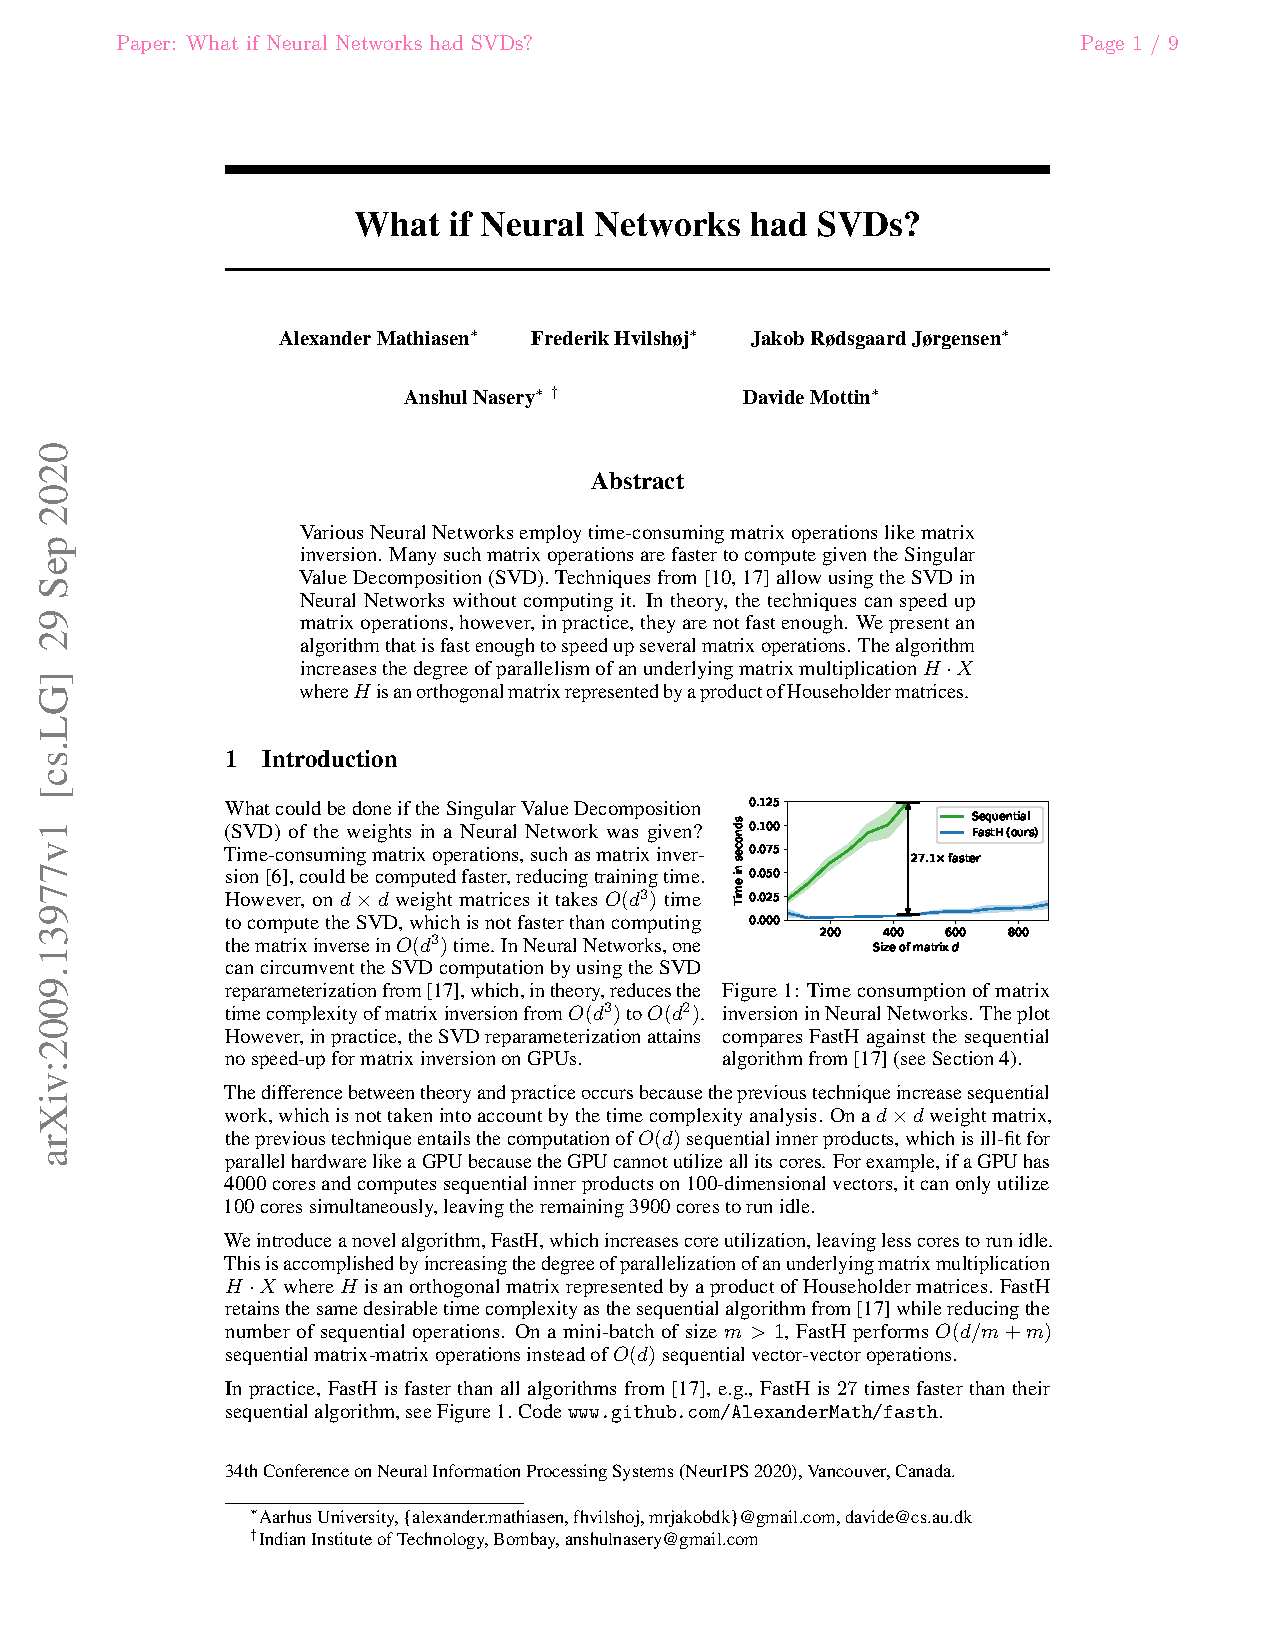
\includepdf[pages=-9]{papers/FastH.pdf}

% One Reflection Suffice
\chapter{One Reflection Suffice}
\label{chap:refl}
\chapterprecishere{\todo{\dots}}
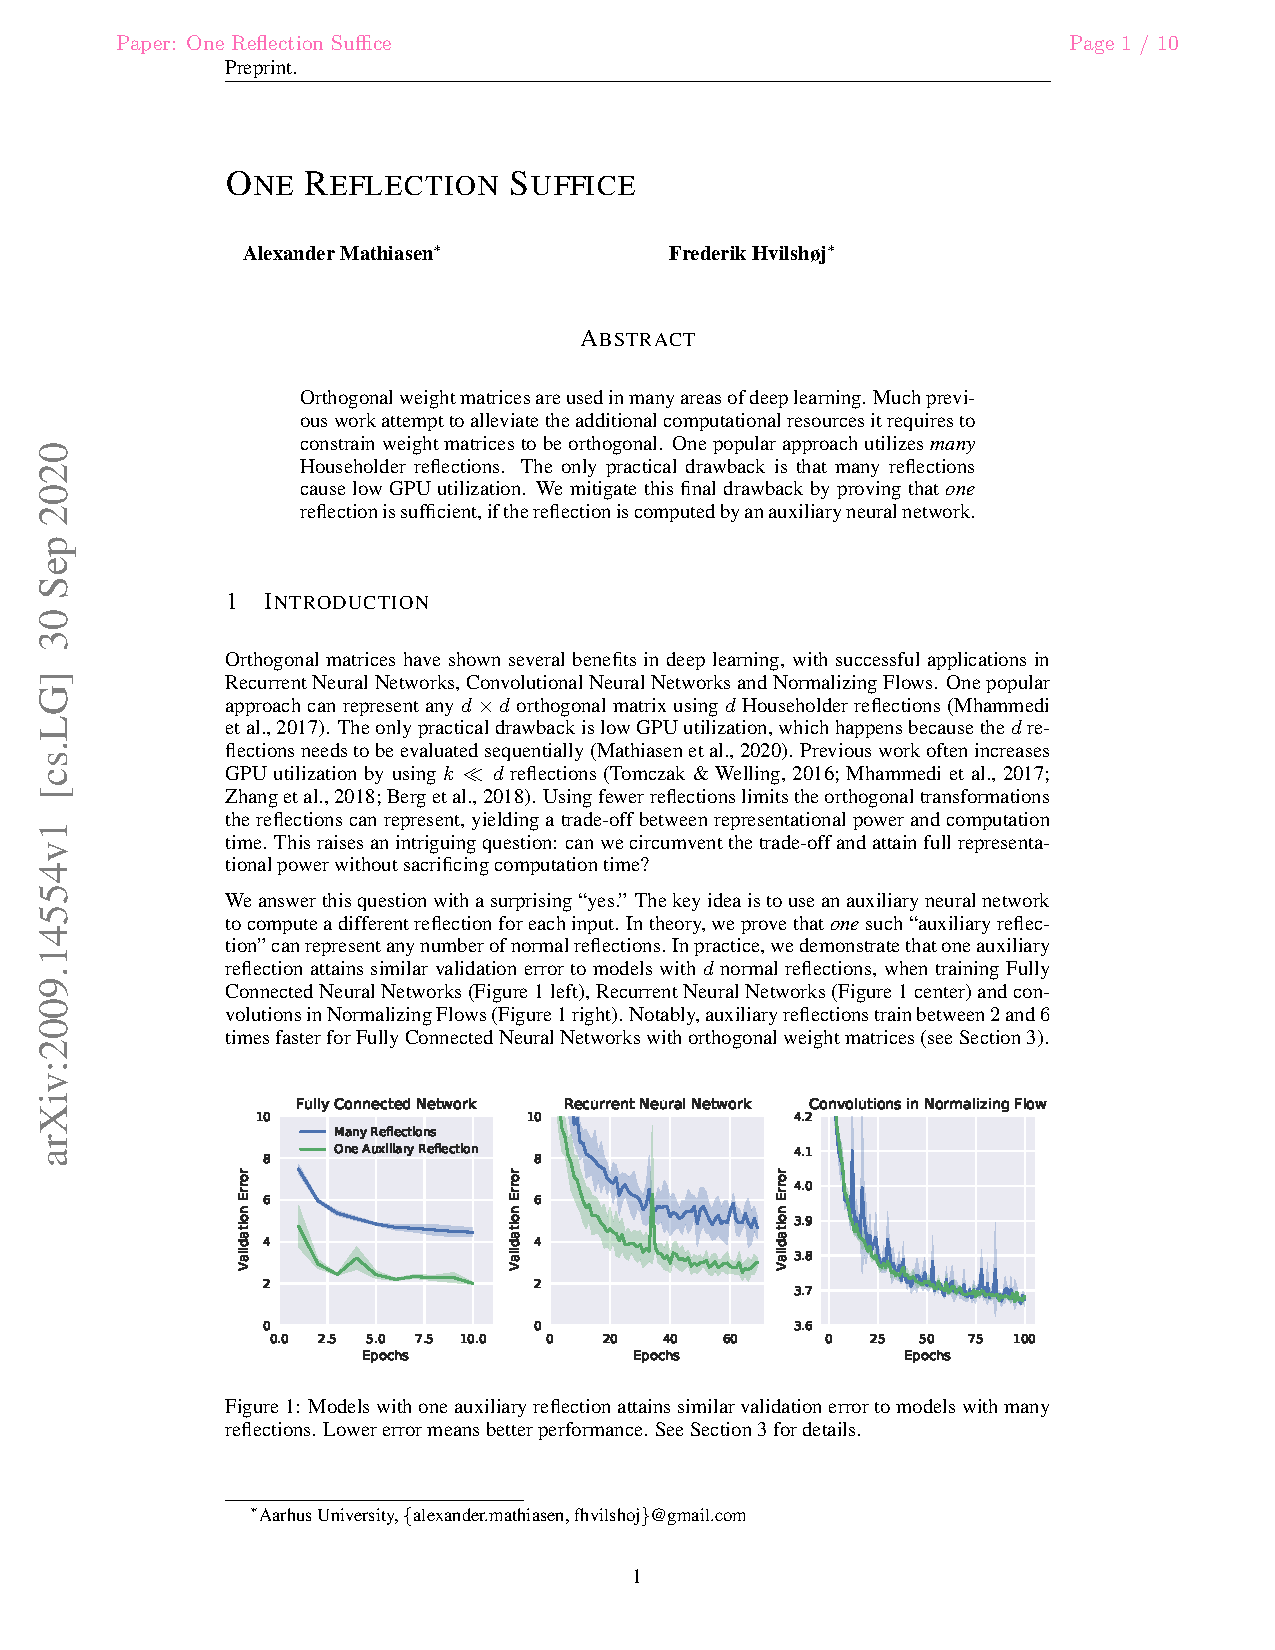
\includepdf[pages=-10]{papers/Refl.pdf}

% FastFID
\chapter{Fast Freché Inception Distance}
\label{chap:fastfid}
\chapterprecishere{\todo{\dots}}
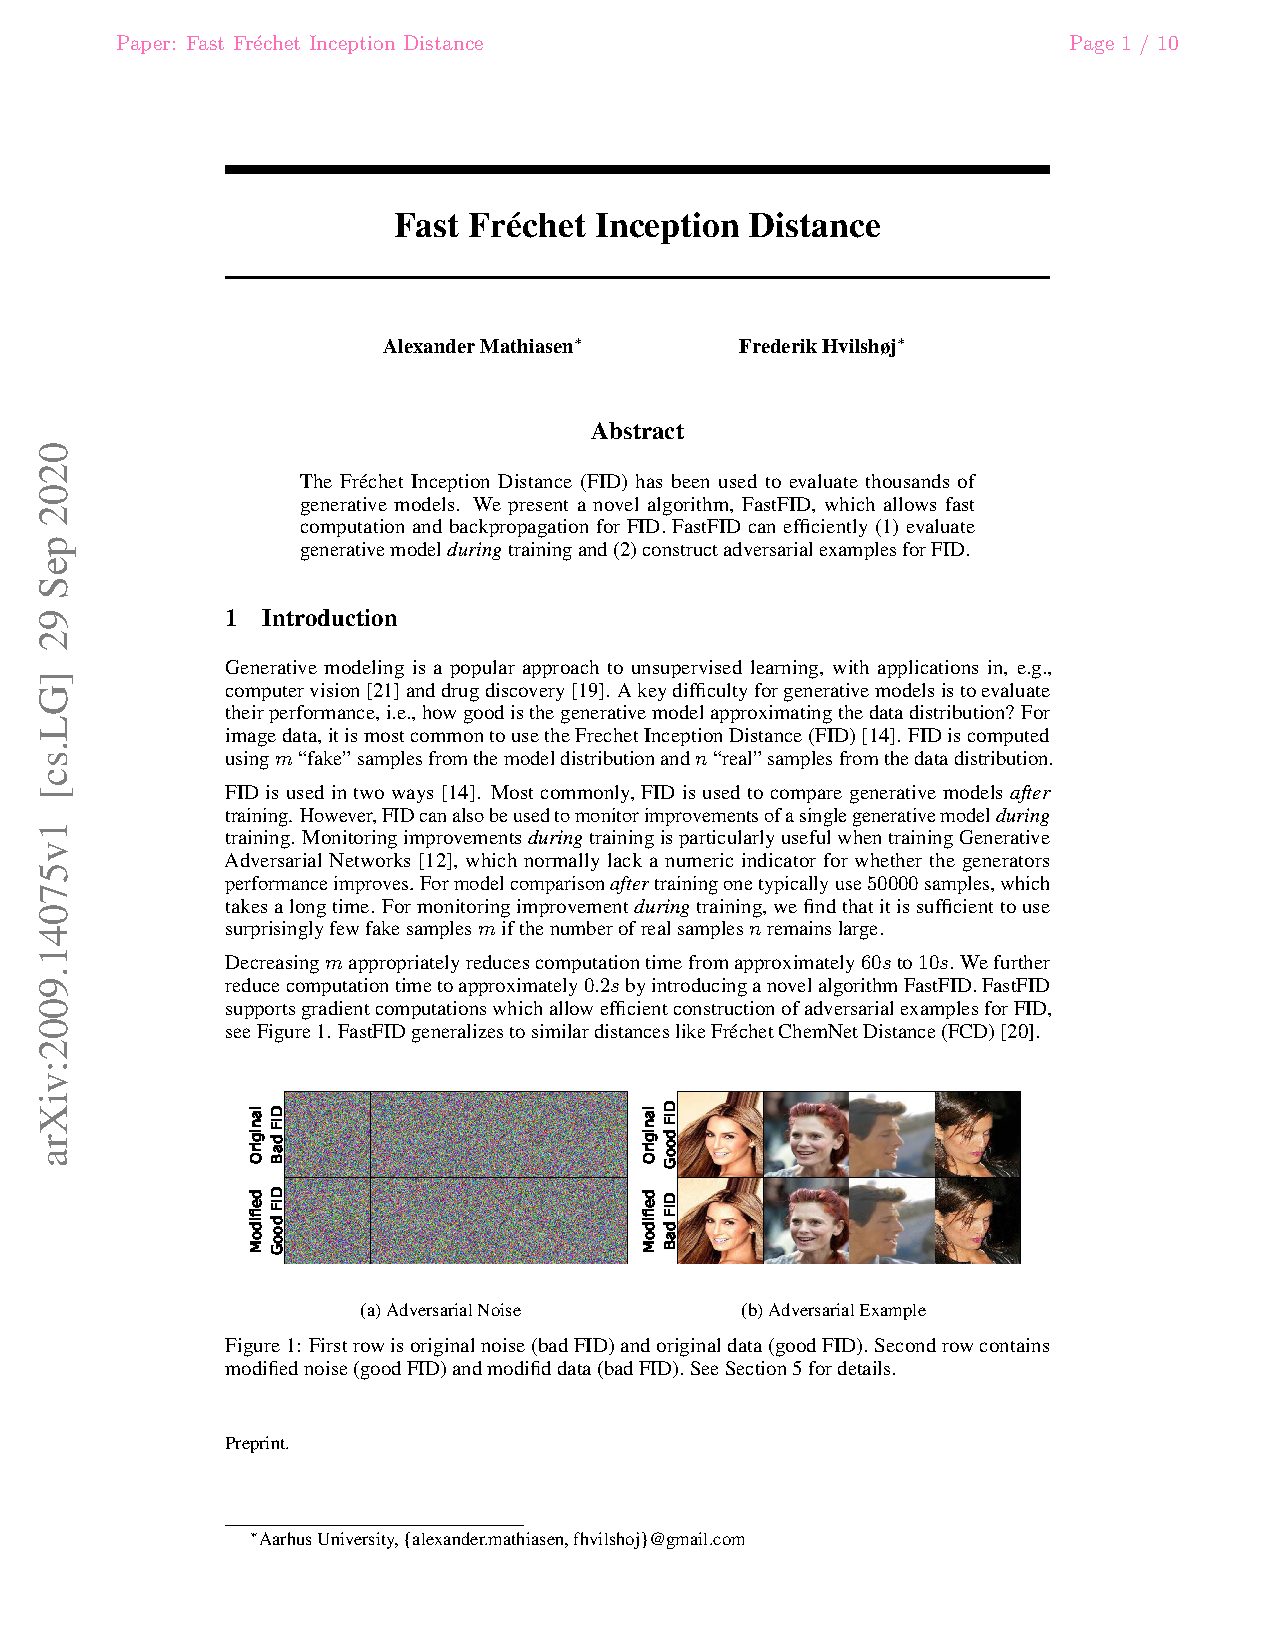
\includepdf[pages=-10]{papers/FastFID.pdf}

% ECINN
\chapter{ECINN: Efficient Counterfactuals from Invertible Neural Networks}
\label{chap:ecinn}
\chapterprecishere{\todo{\dots}}
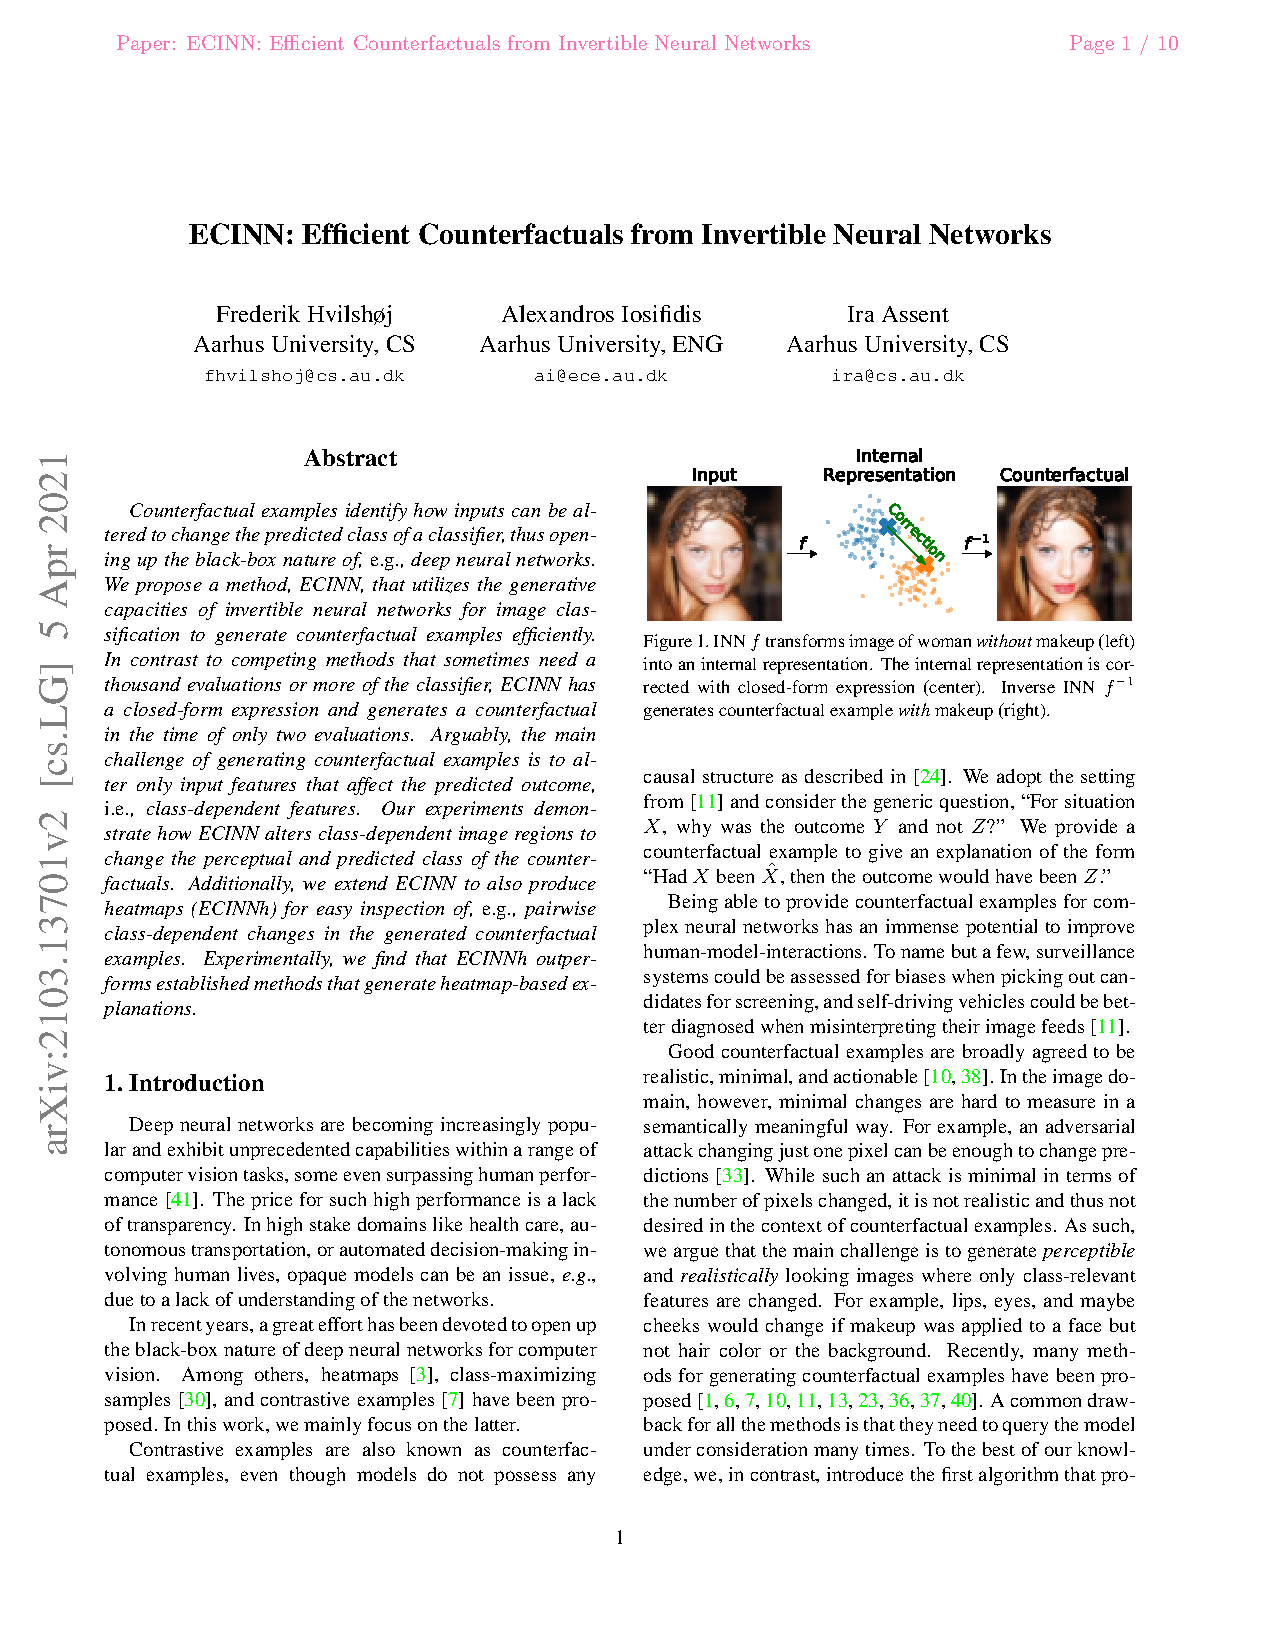
\includepdf[pages=-10]{papers/ECINN.pdf}



\backmatter

%%%%%%%%%%%%%%%%%%%%%%%%%%%%%%%%%%%%%%%%%%%%%%%%%%%%%%%%%%%%%%%%%%%%%%%%%%%%%
%% The appendix
%%%%%%%%%%%%%%%%%%%%%%%%%%%%%%%%%%%%%%%%%%%%%%%%%%%%%%%%%%%%%%%%%%%%%%%%%%%%%
% \part{Appendix}
% \appendix

%%%%%%%%%%%%%%%%%%%%%%%%%%%%%%%%%%%%%%%%%%%%%%%%%%%%%%%%%%%%%%%%%%%%%%%%%%%%%
%% The bibliography
%%%%%%%%%%%%%%%%%%%%%%%%%%%%%%%%%%%%%%%%%%%%%%%%%%%%%%%%%%%%%%%%%%%%%%%%%%%%%

\cleardoublepage
\bibliographystyle{plainnat} 
\bibliography{bibliography}

\end{document}
